\documentclass[lettersize,journal]{IEEEtran}
\usepackage{amsmath,amsfonts}
\usepackage{algorithmic}
\usepackage{algorithm}
\usepackage{array}
\usepackage[caption=false,font=normalsize,labelfont=sf,textfont=sf]{subfig}
\usepackage{textcomp}
\usepackage{stfloats}
\usepackage{url}
\usepackage{verbatim}
\usepackage{graphicx}
\usepackage{cite}
\hyphenation{op-tical net-works}

\begin{document}

\title{Neural Networks-Deep Learning \\ 1st Assignment}
\author{Papadakis Konstantinos Fotios}
% The paper headers
\markboth{Neural Networks-Deep Learning, 1st Assignment, 2024}
\maketitle

\begin{abstract}
This is the first Assignment of the course "Neural Networks-Deep Learning". It is split into two parts.
The first part requires solving our classification problem using KNN and Nearest Centroid classifiers and 
the second part realizes the limitation of the first part's implementation to devise a approach. This 
approach consists of formulating a feed-forward neural network (either MLP, CNN or a combination of both)
which will be trained through a back-propagation algorithm.
\end{abstract}

\section{Introduction}

\IEEEPARstart{T}{he} dataset we are going to be using throughout the assignment is "CIFAR-10".
\begin{itemize}
  \item \url{https://www.cs.toronto.edu/~kriz/cifar.html}
\end{itemize}

It consists of 60000 32x32 color images which belong to one of the 10 available classes. There are 
60000 images per class, 50000 training images and 10000 test images. The data is available in batches of 
10000 images each.
\begin{itemize}
  \item five training batches (or 5000 images from each class)
  \item one test batch (or 1000 images from each class)
\end{itemize}
Since the training batches' images are chosen randomly, each batch individually may contain more images 
from one class than another but, cumulatively, the number of images from each class is equal. 
Here is an example of the dataset's structure:

\begin{figure}[H]
  \centering
  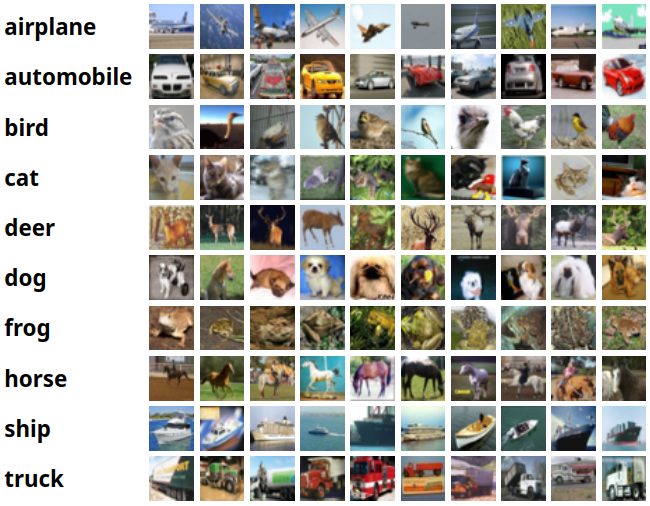
\includegraphics[width=2.5in]{cifar10_example.png}
  \caption{The CIFAR-10 dataset.}
  \label{CIFAR example}
\end{figure}

\section{KNN and Nearest Centroid Classifiers}
In these simple training algorithms the training data is stored as 3D image tensors (32x32x3) 
which we flatten into 1D arrays of 3072 elements(features). These arrays are later used to calculate 
one of two things:
\begin{itemize}
  \item Either the 1 nearest image from the training images (and the majority of the 3 nearest images)
  \item Or the distance between the test image and the centroid of the training images' classes.
\end{itemize}
The code included (cifar10knncentroid.py) is extensively documented and contains key information 
as comments. 

Here are some results from a test run using a subset of the data:
\begin{verbatim}
Loading and preparing CIFAR-10 dataset...
Files already downloaded and verified
Files already downloaded and verified

Evaluating KNN (k=1)...

KNN (k=1) Results:
Training time: 0.36 seconds
Accuracy: 0.2680

Detailed Classification Report:
              precision    recall  f1-score   support

           0       0.27      0.33      0.30       103
           1       0.55      0.13      0.22        89
           2       0.19      0.37      0.26       100
           3       0.28      0.18      0.22       103
           4       0.15      0.39      0.22        90
           5       0.21      0.15      0.18        86
           6       0.29      0.25      0.27       112
           7       0.47      0.18      0.26       102
           8       0.42      0.56      0.48       106
           9       0.54      0.12      0.20       109

    accuracy                           0.27      1000
   macro avg       0.34      0.27      0.26      1000
weighted avg       0.34      0.27      0.26      1000


Evaluating KNN (k=3)...

KNN (k=3) Results:
Training time: 0.33 seconds
Accuracy: 0.2610

Detailed Classification Report:
              precision    recall  f1-score   support

           0       0.27      0.55      0.36       103
           1       0.41      0.16      0.23        89
           2       0.17      0.45      0.25       100
           3       0.29      0.17      0.22       103
           4       0.15      0.33      0.21        90
           5       0.17      0.07      0.10        86
           6       0.37      0.20      0.26       112
           7       0.60      0.09      0.15       102
           8       0.49      0.52      0.50       106
           9       0.56      0.05      0.08       109

    accuracy                           0.26      1000
   macro avg       0.35      0.26      0.24      1000
weighted avg       0.35      0.26      0.24      1000


Evaluating Nearest Centroid...

Nearest Centroid Results:
Training time: 0.03 seconds
Accuracy: 0.2910

Detailed Classification Report:
              precision    recall  f1-score   support

           0       0.26      0.50      0.34       103
           1       0.33      0.24      0.27        89
           2       0.23      0.11      0.15       100
           3       0.12      0.02      0.03       103
           4       0.18      0.08      0.11        90
           5       0.19      0.22      0.20        86
           6       0.26      0.54      0.35       112
           7       0.32      0.20      0.24       102
           8       0.50      0.42      0.46       106
           9       0.36      0.49      0.42       109

    accuracy                           0.29      1000
   macro avg       0.28      0.28      0.26      1000
weighted avg       0.28      0.29      0.26      1000


Performance Comparison:
Classifier           Accuracy   Training Time (s)
---------------------------------------------
KNN (k=1)            0.2680    0.36
KNN (k=3)            0.2610    0.33
Nearest Centroid     0.2910    0.03
\end{verbatim}

\vfill

\end{document}


